\documentclass[14pt]{extbook}
\usepackage{multicol, enumerate, enumitem, hyperref, color, soul, setspace, parskip, fancyhdr} %General Packages
\usepackage{amssymb, amsthm, amsmath, bbm, latexsym, units, mathtools} %Math Packages
\everymath{\displaystyle} %All math in Display Style
% Packages with additional options
\usepackage[headsep=0.5cm,headheight=12pt, left=1 in,right= 1 in,top= 1 in,bottom= 1 in]{geometry}
\usepackage[usenames,dvipsnames]{xcolor}
\usepackage{dashrule}  % Package to use the command below to create lines between items
\newcommand{\litem}[1]{\item#1\hspace*{-1cm}\rule{\textwidth}{0.4pt}}
\pagestyle{fancy}
\lhead{Progress Quiz 8}
\chead{}
\rhead{Version C}
\lfoot{4553-3922}
\cfoot{}
\rfoot{Fall 2020}
\begin{document}

\begin{enumerate}
\litem{
Solve the radical equation below. Then, choose the interval(s) that the solution(s) belongs to.\[ \sqrt{6 x + 2} - \sqrt{9 x - 5} = 0 \]\begin{enumerate}[label=\Alph*.]
\item \( x_1 \in [-0.62, 0.68] \text{ and } x_2 \in [1.9,2.6] \)
\item \( x_1 \in [-0.62, 0.68] \text{ and } x_2 \in [-1.9,1.7] \)
\item \( x \in [2.13,2.47] \)
\item \( \text{All solutions lead to invalid or complex values in the equation.} \)
\item \( x \in [-1.77,-0.52] \)

\end{enumerate} }
\litem{
What is the domain of the function below?\[ f(x) = \sqrt[6]{-9 x - 7} \]\begin{enumerate}[label=\Alph*.]
\item \( [a, \infty), \text{where } a \in [-0.83, -0.54] \)
\item \( (-\infty, a], \text{ where } a \in [-0.9, 0.6] \)
\item \( (-\infty, a], \text{where } a \in [-2.5, -1] \)
\item \( [a, \infty), \text{where } a \in [-1.92, -1.26] \)
\item \( (-\infty, \infty) \)

\end{enumerate} }
\litem{
Solve the radical equation below. Then, choose the interval(s) that the solution(s) belongs to.\[ \sqrt{18 x^2 - 18} - \sqrt{-15 x} = 0 \]\begin{enumerate}[label=\Alph*.]
\item \( \text{All solutions lead to invalid or complex values in the equation.} \)
\item \( x \in [-7.5,-0.5] \)
\item \( x_1 \in [-1.33, 8.67] \text{ and } x_2 \in [0.78,2.33] \)
\item \( x \in [-1.33,8.67] \)
\item \( x_1 \in [-7.5, -0.5] \text{ and } x_2 \in [0.45,0.76] \)

\end{enumerate} }
\litem{
Solve the radical equation below. Then, choose the interval(s) that the solution(s) belongs to.\[ \sqrt{-20 x^2 - 54} - \sqrt{66 x} = 0 \]\begin{enumerate}[label=\Alph*.]
\item \( \text{All solutions lead to invalid or complex values in the equation.} \)
\item \( x \in [-1.64,-1.31] \)
\item \( x_1 \in [-2.05, -1.67] \text{ and } x_2 \in [-3,-1.1] \)
\item \( x \in [-2.05,-1.67] \)
\item \( x_1 \in [1.51, 1.85] \text{ and } x_2 \in [-1.1,3.6] \)

\end{enumerate} }
\litem{
Choose the graph of the equation below.\[ f(x) = \sqrt{x + 12} - 4 \]\begin{enumerate}[label=\Alph*.]
\begin{multicols}{2}\item 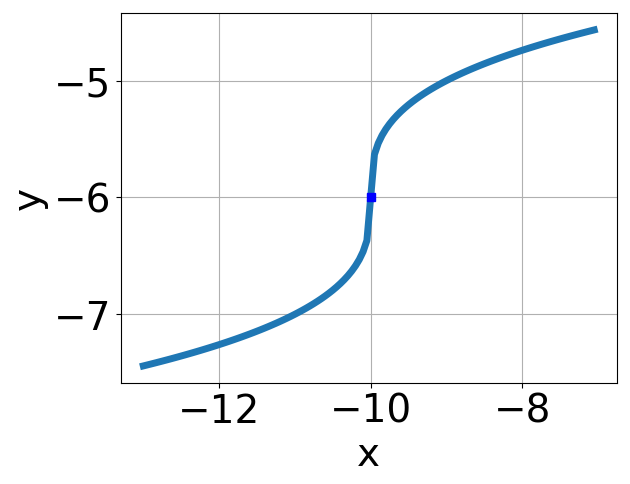
\includegraphics[width = 0.3\textwidth]{../Figures/radicalEquationToGraphAC.png}\item 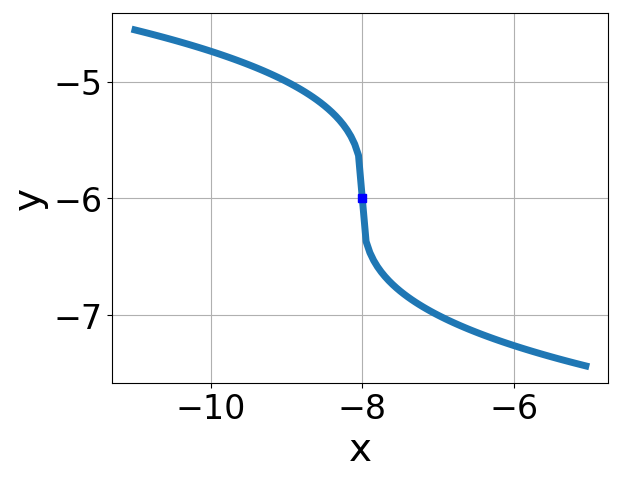
\includegraphics[width = 0.3\textwidth]{../Figures/radicalEquationToGraphBC.png}\item 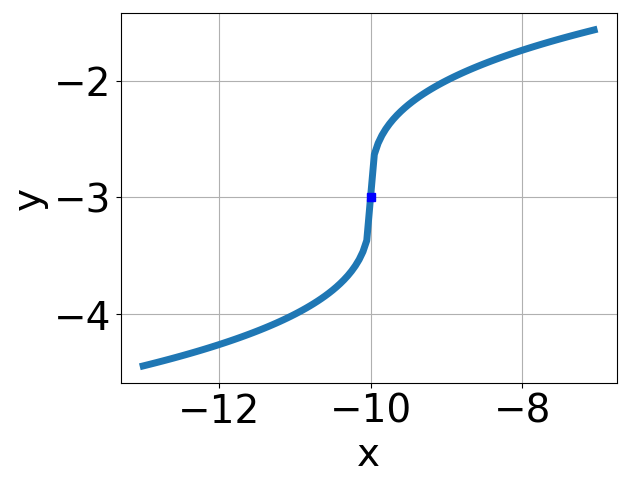
\includegraphics[width = 0.3\textwidth]{../Figures/radicalEquationToGraphCC.png}\item 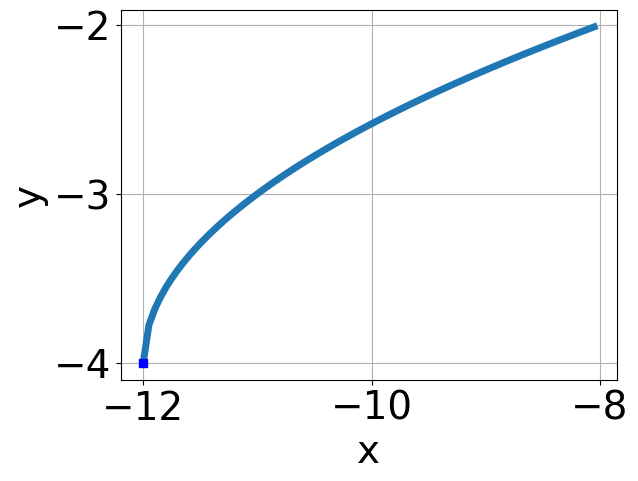
\includegraphics[width = 0.3\textwidth]{../Figures/radicalEquationToGraphDC.png}\end{multicols}\item None of the above.
\end{enumerate} }
\litem{
Choose the equation of the function graphed below.
\begin{center}
    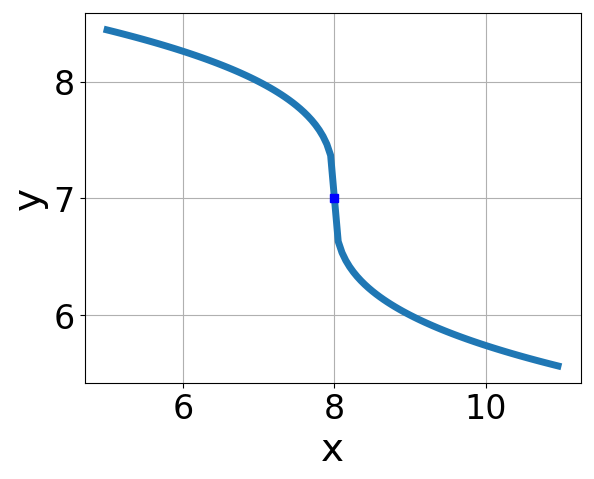
\includegraphics[width=0.5\textwidth]{../Figures/radicalGraphToEquationC.png}
\end{center}
\begin{enumerate}[label=\Alph*.]
\item \( f(x) = \sqrt[3]{x - 12} + 6 \)
\item \( f(x) = \sqrt[3]{x + 12} + 6 \)
\item \( f(x) = - \sqrt[3]{x + 12} + 6 \)
\item \( f(x) = - \sqrt[3]{x - 12} + 6 \)
\item \( \text{None of the above} \)

\end{enumerate} }
\litem{
Solve the radical equation below. Then, choose the interval(s) that the solution(s) belongs to.\[ \sqrt{7 x - 6} - \sqrt{-9 x + 6} = 0 \]\begin{enumerate}[label=\Alph*.]
\item \( x_1 \in [0.65, 0.73] \text{ and } x_2 \in [-3.14,1.86] \)
\item \( x_1 \in [0.74, 0.81] \text{ and } x_2 \in [-3.14,1.86] \)
\item \( \text{All solutions lead to invalid or complex values in the equation.} \)
\item \( x \in [0.74,0.81] \)
\item \( x \in [-0.03,0.05] \)

\end{enumerate} }
\litem{
Choose the equation of the function graphed below.
\begin{center}
    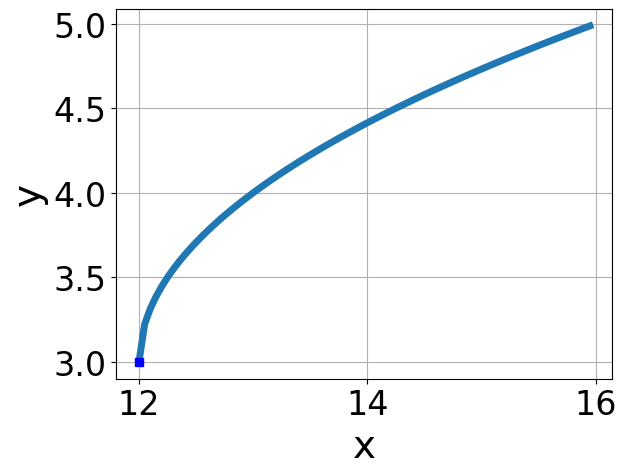
\includegraphics[width=0.5\textwidth]{../Figures/radicalGraphToEquationCopyC.png}
\end{center}
\begin{enumerate}[label=\Alph*.]
\item \( f(x) = \sqrt{x + 14} - 3 \)
\item \( f(x) = - \sqrt{x - 14} - 3 \)
\item \( f(x) = \sqrt{x - 14} - 3 \)
\item \( f(x) = - \sqrt{x + 14} - 3 \)
\item \( \text{None of the above} \)

\end{enumerate} }
\litem{
Choose the graph of the equation below.\[ f(x) = - \sqrt[3]{x + 12} + 4 \]\begin{enumerate}[label=\Alph*.]
\begin{multicols}{2}\item 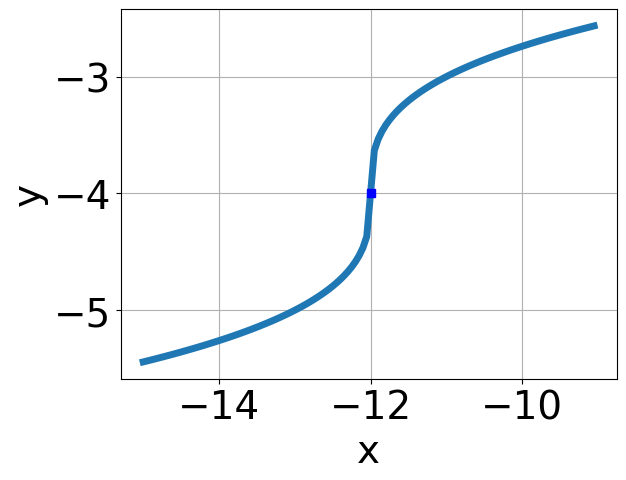
\includegraphics[width = 0.3\textwidth]{../Figures/radicalEquationToGraphCopyAC.png}\item 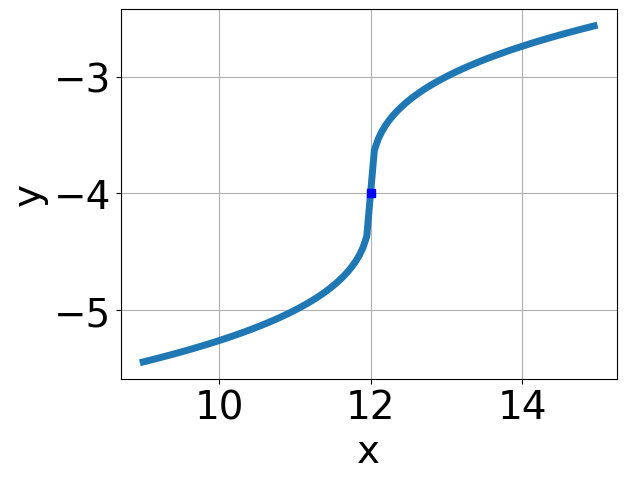
\includegraphics[width = 0.3\textwidth]{../Figures/radicalEquationToGraphCopyBC.png}\item 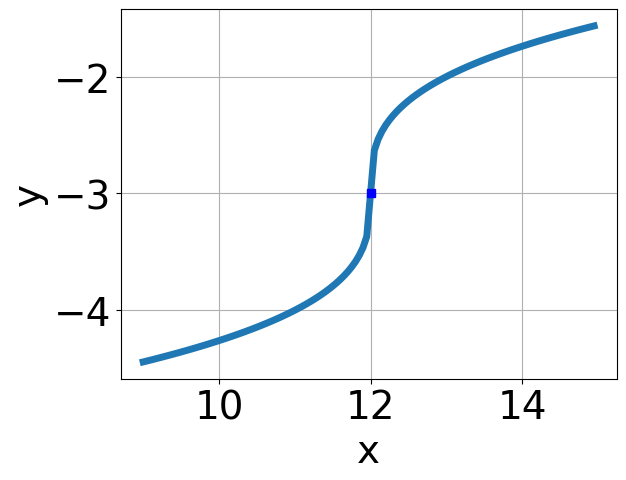
\includegraphics[width = 0.3\textwidth]{../Figures/radicalEquationToGraphCopyCC.png}\item 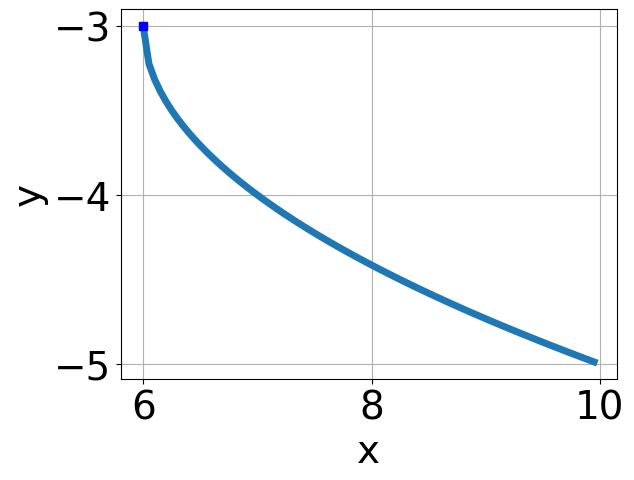
\includegraphics[width = 0.3\textwidth]{../Figures/radicalEquationToGraphCopyDC.png}\end{multicols}\item None of the above.
\end{enumerate} }
\litem{
What is the domain of the function below?\[ f(x) = \sqrt[8]{3 x + 8} \]\begin{enumerate}[label=\Alph*.]
\item \( (-\infty, a], \text{where } a \in [-0.8, 2.8] \)
\item \( [a, \infty), \text{ where } a \in [-5.1, -1.7] \)
\item \( [a, \infty), \text{where } a \in [-1, 1.4] \)
\item \( (-\infty, a], \text{where } a \in [-3.7, -1.4] \)
\item \( (-\infty, \infty) \)

\end{enumerate} }
\end{enumerate}

\end{document}